\documentclass[11pt,a4paper]{article}
\usepackage{gtu-el-yazisi}
\begin{document}
\notbilgi{Alan Teorisi}{Uygulama 9 -- Görüntü yöntemi (köşe, dielektrik arayüz)}{Uygulama-9.pdf}
% yerel yardımcı: üstü çizili (sadeleştirilen) terimler
\newcommand\iptalX[3]{\tikz[baseline=(c.base)]{\node[inner sep=0pt](c){$#2#3$};\draw[#1,line width=0.5pt](c.south west)--(c.north east);}}
\newcommand\iptalK[2]{\iptalX{murekkep}{#1}{#2}}
\newcommand\iptalO[2]{\iptalX{turuncukalem}{#1}{#2}}
\newcommand\iptalR[2]{\iptalX{kirmizikalem}{#1}{#2}}
\newcommand\iptal[1]{\mathpalette\iptalK{#1}}
\newcommand\iptalt[1]{\mathpalette\iptalO{#1}}
\newcommand\iptalk[1]{\mathpalette\iptalR{#1}}

\sayfa{1}
\begin{center}\textcolor{kirmizikalem}{\underline{görüntü teoremi}}\end{center}
\noindent\textcolor{kirmizikalem}{\underline{S65 Pr.6}}

\noindent
\begin{minipage}[c]{0.60\linewidth}
\begin{tikzpicture}[line width=0.8pt]
  \draw[-{Stealth}] (0,0) -- (0,3.6) node[right] {$y$};
  \draw[-{Stealth}] (0,0) -- (5.7,0) node[right] {$x$};
  \foreach \hy in {0.3,0.65,...,3.2} \draw[line width=0.6pt] (0,\hy) -- ++(-0.2,-0.25);
  \foreach \hx in {0.3,0.75,...,5.2} \draw[line width=0.6pt] (\hx,0) -- ++(-0.2,-0.25);
  \draw[dashed] (0,1.9) -- (2.2,1.9) -- (2.2,0);
  \fill (2.2,1.9) circle (1.3pt);
  \node[right] at (2.25,1.9) {$q$};
  \node[above right] at (0,1.9) {$b$};
  \node[above right] at (2.2,0) {$a$};
\end{tikzpicture}
\end{minipage}\hfill
\begin{minipage}[c]{0.36\linewidth}
$q$ yüküne\\ etki eden kuvvet
\end{minipage}

\begin{center}
\begin{tikzpicture}[line width=0.8pt,scale=0.9]
  \draw[turuncukalem,-{Stealth}] (0,0) -- (-4.3,0);
  \draw[turuncukalem,-{Stealth}] (0,0) -- (0,-3.4);
  \draw[-{Stealth}] (0,0) -- (0,3.6) node[right] {$y$};
  \draw[-{Stealth}] (0,0) -- (5.7,0) node[right] {$x$};
  \foreach \hy in {0.3,0.7,...,3.0} \draw[line width=0.6pt] (0,\hy) -- ++(-0.2,-0.25);
  \foreach \hx in {0.3,0.8,...,5.2} \draw[line width=0.6pt] (\hx,0) -- ++(-0.2,-0.25);
  \draw[dashed] (0,1.93) -- (1.9,1.93) -- (1.9,0);
  \draw[turuncukalem,dashed] (0,1.93) -- (-1.93,1.93) -- (-1.93,-1.87) -- (1.9,-1.87) -- (1.9,0);
  \draw[dashed] (-1.93,-1.87) -- (1.9,1.93);
  \fill (1.9,1.93) circle (1.5pt);
  \fill[turuncukalem] (-1.93,1.93) circle (1.5pt);
  \fill[turuncukalem] (-1.93,-1.87) circle (1.5pt);
  \fill[turuncukalem] (1.9,-1.87) circle (1.5pt);
  \node[right] at (1.95,2.0) {$q\ (a,b)$};
  \node[turuncukalem,left] at (-1.95,1.95) {$-q$};
  \node[turuncukalem,right] at (1.95,-1.85) {$-q$};
  \node[turuncukalem,left] at (-1.95,-1.85) {$+q$};
  \node[below] at (-1.2,-2.0) {$(-a,-b)$};
  \node[turuncukalem] at (-1.93,-0.3) {$-a$};
  \node[turuncukalem] at (0.5,-1.65) {$-b$};
  \node at (0.25,2.15) {$b$};
  \node at (1.95,0.25) {$a$};
  \draw[kirmizikalem,-{Stealth}] (0.15,0.5) -- (0.75,1.1);
  \node[kirmizikalem] at (0.45,0.35) {$r$};
\end{tikzpicture}
\end{center}

\begin{align*}
\vec F &= -\frac{q^2}{4\pi\varepsilon\,4a^2}\,\vec e_x-\frac{q^2}{4\pi\varepsilon\,4b^2}\,\vec e_y \\
&\quad+\frac{q^2}{4\pi\varepsilon\,2\sqrt{a^2+b^2}}\left(\frac{a\vec e_x+b\vec e_y}{\sqrt{a^2+b^2}}\right)\footnotemark
\end{align*}
\footnotetext{Claude notu: muhtemelen payda $4\pi\varepsilon\,\bigl(2\sqrt{a^2+b^2}\bigr)^2$ olmalı (son satırdaki $16\pi\varepsilon$ ile uyumlu).}
\[ \textcolor{kirmizikalem}{|\vec r|=2\sqrt{a^2+b^2}} \]
\[ \textcolor{kirmizikalem}{\vec e_r=\frac{\vec r}{|\vec r|}=\frac{2a\,\vec e_x+2b\,\vec e_y}{2\sqrt{a^2+b^2}}=\frac{a\,\vec e_x+b\,\vec e_y}{\sqrt{a^2+b^2}}} \]
\[ \vec F=\frac{q^2}{16\pi\varepsilon}\left[\vec e_x\left(-\frac{1}{a^2}+\frac{a}{(a^2+b^2)^{3/2}}\right)+\vec e_y\left(-\frac{1}{b^2}+\frac{b}{(a^2+b^2)^{3/2}}\right)\right] \]

\begin{minipage}{\linewidth}
\noindent\textcolor{kirmizikalem}{\underline{S66 Pr.7}}
\begin{center}
\begin{tikzpicture}[line width=0.8pt]
  \draw[-{Stealth}] (0,0) -- (0,3.0) node[right] {$y$};
  \draw[-{Stealth}] (0,0) -- (5.2,0) node[right] {$x$};
  \foreach \hy in {0.3,0.65,...,2.6} \draw[line width=0.6pt] (0,\hy) -- ++(-0.2,-0.25);
  \foreach \hx in {0.3,0.65,...,4.6} \draw[line width=0.6pt] (\hx,0) -- ++(-0.2,-0.25);
  \draw[dashed] (0,1.9) -- (2.1,1.9);
  \draw[dashed] (2.2,1.9) -- (2.2,0);
  \fill (2.2,1.9) circle (1.3pt);
  \node[right] at (2.35,1.95) {$\rho_c$};
  \node[left] at (0,1.9) {$b$};
  \node[above right] at (2.2,0) {$a$};
  \draw[-{Stealth}] (2.9,2.15) -- (3.35,2.5);
  \node[anchor=west,align=left] at (3.4,2.3) {z ekseni\\ boyunca\\ eksi sonsuzdan\\ sonsuza};
\end{tikzpicture}
\end{center}
\noindent $\rho_c$'nin birim uzunluğuna etki\\
eden kuvvet nedir?
\end{minipage}

\sayfa{2}
\begin{center}
\begin{tikzpicture}[line width=0.8pt]
  \draw[turuncukalem,-{Stealth}] (0,0) -- (-2.6,0) ;
  \draw[turuncukalem] (0,0) -- (0,-3.2);
  \draw[-{Stealth}] (0,0) -- (0,2.8) node[right] {$y$};
  \draw[-{Stealth}] (0,0) -- (5.2,0) node[right] {$x$};
  \foreach \hy in {0.3,0.65,...,1.8} \draw[line width=0.6pt] (0,\hy) -- ++(-0.2,-0.25);
  \foreach \hx in {0.3,0.65,...,4.6} \draw[line width=0.6pt] (\hx,0) -- ++(-0.2,-0.25);
  \draw[dashed] (0,1.9) -- (1.9,1.9);
  \draw[dashed] (1.98,1.9) -- (1.98,0);
  \fill (1.98,1.9) circle (1.3pt);
  \node[right] at (2.1,1.95) {$\rho_c$};
  \node[left] at (0,1.9) {$b$};
  \node[above right] at (1.98,0) {$a$};
  \draw[turuncukalem,dashed] (0,1.9) -- (-1.93,1.9) -- (-1.93,-1.85) -- (1.98,-1.85) -- (1.98,0);
  \node[turuncukalem,left] at (-1.95,1.9) {$-\rho_c$};
  \node[turuncukalem] at (-1.93,-0.3) {$-a$};
  \node[turuncukalem] at (-0.4,-2.1) {$-b$};
  \node[turuncukalem,right] at (2.0,-2.1) {$-\rho_c$};
  \draw[-{Stealth}] (2.7,2.15) -- (3.2,2.5);
  \node[anchor=west,align=left] at (3.25,2.3) {z ekseni\\ boyunca\\ eksi sonsuzdan\\ sonsuza};
\end{tikzpicture}
\end{center}

\begin{center}
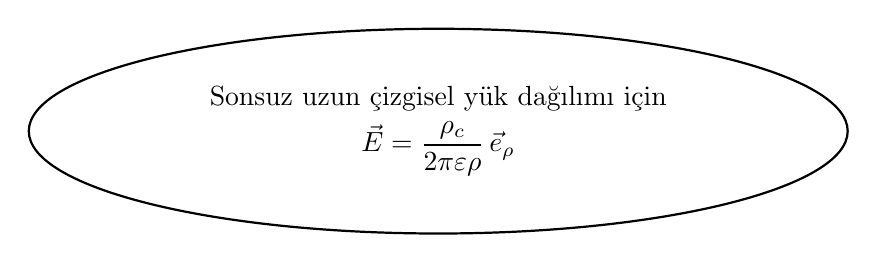
\begin{tikzpicture}
  \node[align=center](c){Sonsuz uzun çizgisel yük dağılımı için\\[1mm] $\displaystyle\vec E=\frac{\rho_c}{2\pi\varepsilon\rho}\,\vec e_\rho$};
  \draw[line width=0.8pt] (c.center) ellipse (5.2cm and 1.3cm);
\end{tikzpicture}
\end{center}

\[ \vec E=-\frac{\rho_c}{2\pi\varepsilon\,2a}\,\vec e_x-\frac{\rho_c}{2\pi\varepsilon\,2b}\,\vec e_y+\frac{\rho_c}{2\pi\varepsilon\,2\sqrt{a^2+b^2}}\left(\frac{a\vec e_x+b\vec e_y}{\sqrt{a^2+b^2}}\right) \]
\[ \vec E=\frac{\rho_c}{4\pi\varepsilon}\left(\vec e_x\left(-\frac{1}{a}+\frac{a}{a^2+b^2}\right)+\vec e_y\left(-\frac{1}{b}+\frac{b}{a^2+b^2}\right)\right) \]
\[ =-\frac{\rho_c}{4\pi\varepsilon(a^2+b^2)}\left[+\vec e_x\,\frac{b^2}{a}+\vec e_y\,\frac{a^2}{b}\right] \]
\begin{align*}
\vec F &= \int_{z=0}^{z=1}\rho_c\,\vec E\,dz=\rho_c\vec E \\
&= -\frac{\rho_c^2}{4\pi\varepsilon(a^2+b^2)}\left[+\vec e_x\,\frac{b^2}{a}+\vec e_y\,\frac{a^2}{b}\right]
\end{align*}

\begin{minipage}{\linewidth}
\noindent\textcolor{kirmizikalem}{\underline{S66 Pr.8}}
\begin{center}
\begin{tikzpicture}[line width=0.8pt,scale=0.9]
  \draw[-{Stealth}] (0,0) -- (0,3.7) node[right] {$z$};
  \draw[-{Stealth}] (-3.7,0) -- (6.1,0) node[right] {$x$};
  \node at (0.3,0.35) {$O$};
  \node at (-1.9,1.65) {$\varepsilon_1$};
  \node at (-2.1,-1.1) {$\varepsilon_2$};
  \draw[kirmizikalem,dashed] (0,1.9) -- (2.94,1.9);
  \node[kirmizikalem,left] at (0,1.9) {$c$};
  \fill (2.94,1.9) circle (1.3pt);
  \node[above left] at (2.94,1.9) {$M_0$};
  \node[right] at (2.95,1.85) {$q$};
  \node at (4.3,3.1) {$M_0$ noktası};
  \node[kirmizikalem] at (4.5,2.5) {$(a,b,c)$};
  \draw (2.94,1.9) -- (4.87,1.18) node[right] {$M$};
  \node at (4.2,1.95) {$r'$};
  \draw[dotted] (2.94,1.9) -- (2.94,0);
  \draw[turuncukalem,dashed] (2.94,0) -- (2.94,-1.93);
  \fill[turuncukalem] (2.94,-1.93) circle (1.3pt);
  \node[turuncukalem,left] at (2.9,-1.95) {$M_1$};
  \draw[turuncukalem] (4.87,1.18) -- (2.94,-1.93);
  \node[turuncukalem] at (4.2,-0.9) {$r_1'$};
  \node[turuncukalem,right] at (3.1,-1.7) {$\rightarrow$ görüntü yükü};
  \node[turuncukalem] at (2.65,-0.35) {$q$};
\end{tikzpicture}
\end{center}
\noindent
\begin{minipage}[c]{0.27\linewidth}
$q$ yükünün oluşturduğu pot. fonksiyonu
\end{minipage}\hfill
\begin{minipage}[c]{0.71\linewidth}
\[ V(M)=\begin{cases}
\dfrac{q}{4\pi\varepsilon_1 r'}+\dfrac{q(\varepsilon_1-\varepsilon_2)}{4\pi\varepsilon_1(\varepsilon_1+\varepsilon_2)\,r_1'}\,, & z>0 \\[4mm]
\dfrac{2q\varepsilon_2}{4\pi\varepsilon_2(\varepsilon_1+\varepsilon_2)\,r'}\,, & z<0
\end{cases} \]
\end{minipage}
\end{minipage}

\sayfa{3}
\noindent olduğunu gösteriniz

\noindent $z=0$ düzleminde biriken yükü bulunuz.

\medskip
\noindent\vurgu{Denk problem çözülmeden yazılır}
\[ z>0\qquad \colorbox{gtufosfor-sari}{$\displaystyle\Delta V=-\frac{\rho_v}{\varepsilon_1}$}=-\frac{q}{\varepsilon_1}\,\delta(x-a)\,\delta(y-b)\,\delta(z-c) \]
\[ z<0\qquad \Delta V=0 \]
\noindent $z=0$ \qquad \vurgu{sınır problemleri:}
\[ \colorbox{gtufosfor-sari}{$V_1=V_2$}\qquad \colorbox{gtufosfor-sari}{$\vec n\cdot\vec D_1=\vec n\cdot\vec D_2$} \]
\[ \vec e_z\cdot\vec D_1=\vec e_z\cdot\vec D_2 \]
\medskip\hrule\medskip
\noindent Şimdi de denk problemden bakalım

\noindent $z>0$ \qquad $\varepsilon_2=\varepsilon_1$ seçelim

\begin{center}
\begin{tikzpicture}[line width=0.8pt,scale=0.9]
  \draw[-{Stealth}] (0,0) -- (0,3.9) node[right] {$z$};
  \draw[-{Stealth}] (-3.7,0) -- (6.0,0) node[right] {$x$};
  \node at (0.3,0.4) {$O$};
  \node at (-2.0,1.7) {$\varepsilon_1$};
  \node at (-2.1,-1.1) {$\varepsilon_2$};
  \draw[kirmizikalem,dashed] (0,1.97) -- (2.88,1.97);
  \node[kirmizikalem,left] at (0,1.97) {$c$};
  \fill (2.88,1.97) circle (1.3pt);
  \node[above left] at (2.88,1.97) {$M_0$};
  \node[right] at (2.9,1.9) {$q$};
  \node at (4.2,3.2) {$M_0$ noktası};
  \node[kirmizikalem] at (4.4,2.55) {$(a,b,c)$};
  \draw[-{Stealth}] (2.88,1.97) -- (6.19,1.02);
  \node at (4.2,1.85) {$r'$};
  \node at (5.85,0.8) {$\vec e\,'$};
  \node at (5.45,1.42) {$M$};
  \draw[dotted] (2.88,1.97) -- (2.88,0);
  \draw[turuncukalem,dashed] (2.88,0) -- (2.92,-1.84);
  \node[turuncukalem] at (2.65,-0.35) {$q$};
  \draw[turuncukalem,-{Stealth}] (2.92,-1.84) -- (5.08,2.03);
  \node[turuncukalem] at (5.45,1.9) {$\vec e_1'$};
  \node[turuncukalem] at (4.0,-0.85) {$r_1'$};
  \node at (2.5,-1.87) {$M_1$};
  \node[turuncukalem,right] at (3.4,-1.55) {$\rightarrow$ görüntü yükü};
  \node at (3.15,-2.2) {\colorbox{gtufosfor-sari}{$\alpha q$}};
  \draw[turuncukalem,-{Stealth}] (0.94,0.05) -- (0.94,0.55);
  \node[turuncukalem,right] at (1.0,0.85) {$\vec n=\vec e_z$};
\end{tikzpicture}
\end{center}

\noindent $M$'nin $z>0$ iken $M$ noktasında kaynaklanan potansiyel
\[ \colorbox{gtufosfor-sari}{$\displaystyle V_1=\frac{q}{4\pi\varepsilon_1 r'}+\frac{\alpha q}{4\pi\varepsilon_1 r_1'}$} \]
\[ \vec E_1=-\mathrm{grad}\,V_1=\frac{q}{4\pi\varepsilon_1}\left(\frac{1}{r'^2}\,\vec e\,'+\frac{\alpha}{r_1'^2}\,\vec e_1'\right) \]
\begin{align*}
V_1\Big|_{z=0} &= \frac{q}{4\pi\varepsilon_1}\left(\frac{1}{r}+\frac{\alpha}{r}\right) \\
&= \frac{q}{4\pi\varepsilon_1 r}\left(\frac{1}{r}+\frac{\alpha}{r}\right)\footnotemark \\
&= \frac{q}{4\pi\varepsilon_1 r}\,(1+\alpha)
\end{align*}
\footnotetext{Claude notu: bu satır bir sonraki satırla tutarlı değil; muhtemelen parantez içi $(1+\alpha)$ olmalı.}

\elcizimi[0.45]{sekiller/uygulama-notlari-Uygulama-9-s3-1.png}[3]

\[ \vec e_z\cdot\vec D_1\Big|_{z=0}\overset{\varepsilon_1\ \text{gider}}{=}\frac{q}{4\pi}\left(\frac{\vec e_z\cdot\vec e\,'|_{z=0}}{r^2}+\frac{\alpha\,\vec e_z\cdot\vec e_1'|_{z=0}}{r^2}\right) \]

\sayfa{4}
\[ =\frac{q}{4\pi r^2}\left(-\cos\theta+\alpha\cos\theta\right) \]
\begin{center}
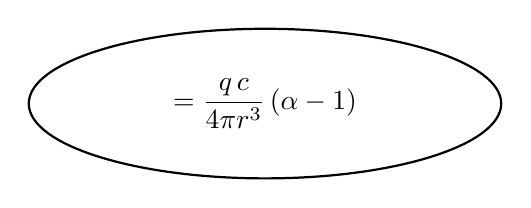
\begin{tikzpicture}
  \node(c){$\displaystyle =\frac{q\,c}{4\pi r^3}\,(\alpha-1)$};
  \draw[line width=0.8pt] (c.center) ellipse (3.0cm and 0.95cm);
\end{tikzpicture}
\end{center}

\noindent $z<0$ bölgesinde $\varepsilon_1=\varepsilon_2=$ olduğunu varsayarak $M_0$'a bir $\beta q$ yükü yerleştirerek denk problemi tanımlayalım

\begin{center}
\begin{tikzpicture}[line width=0.8pt,scale=0.8]
  \draw[-{Stealth}] (0,0) -- (0,3.7) node[right] {$z$};
  \draw[-{Stealth}] (-0.85,0) -- (7.0,0) node[right] {$x$};
  \fill (1.92,1.87) circle (1.3pt);
  \node at (1.37,2.12) {$\beta q$};
  \node at (2.83,2.12) {$M_0$};
  \draw[dashed] (1.92,1.87) -- (1.92,0);
  \draw[-{Stealth}] (1.92,1.87) -- (4.68,-1.02);
  \fill (4.33,-0.64) circle (1.3pt);
  \node at (4.87,-0.3) {$M$};
  \node at (5.0,-0.95) {$\vec e\,'$};
  \node at (3.82,0.8) {$r'$};
  \node at (-0.4,0.85) {$\varepsilon_2$};
  \node at (-0.2,-1.0) {$\varepsilon_2$};
\end{tikzpicture}
\end{center}

\[ V_2=\frac{\beta q}{4\pi\varepsilon_2 r'} \]
\begin{align*}
\vec E=-\mathrm{grad}\,V &= -\frac{\partial V}{\partial r}\,\vec e\,' \\
&= \frac{\beta q}{4\pi\varepsilon_2 r'^2}\,\vec e\,'
\end{align*}
\[ z=0\qquad V_2\Big|_{z}=\frac{\beta q}{4\pi\varepsilon_2 r'} \]

\begin{center}
\begin{tikzpicture}[line width=0.8pt,scale=0.8]
  \draw[-{Stealth}] (0,0) -- (0,3.8) node[right] {$z$};
  \draw[-{Stealth}] (-0.9,0) -- (7.0,0) node[right] {$x$};
  \fill (1.9,1.9) circle (1.3pt);
  \node at (1.33,2.12) {$\beta q$};
  \node at (2.8,2.12) {$M_0$};
  \draw[dashed] (1.9,1.9) -- (1.9,0);
  \draw[-{Stealth}] (1.9,1.9) -- (4.7,-0.99);
  \draw[kirmizikalem] (1.9,1.9) -- (4.98,0.05);
  \fill[kirmizikalem] (4.98,0.05) circle (1.3pt);
  \node[kirmizikalem] at (4.5,1.35) {$r$};
  \node at (4.0,0.85) {$r'$};
  \node[kirmizikalem] at (5.35,0.35) {$M$};
  \node at (4.95,-0.5) {$M$};
  \node at (5.35,-0.95) {$\vec e\,'$};
  \node[turuncukalem] at (2.3,1.3) {$\theta$};
  \node at (-0.4,0.85) {$\varepsilon_2$};
  \node at (-0.2,-1.0) {$\varepsilon_2$};
\end{tikzpicture}
\end{center}

\begin{align*}
\vec e_z\cdot\vec D_2\Big|_{z=0} &= \frac{\beta q}{4\pi r^2}\,\vec e_z\cdot\vec e\,'\Big|_{z=0} \\
&= -\frac{\beta q}{4\pi r^2}\cos\theta \\
&= -\frac{\beta q\,c}{4\pi r^3}
\end{align*}
\[ V_1\Big|_{z=0}=V_2\Big|_{z=0} \]
\[ \frac{\iptal{q}}{\iptal{4\pi}\,\varepsilon_1\,\iptal{r}}\,(1+\alpha)=\frac{\beta\,\iptal{q}}{\iptal{4\pi}\,\varepsilon_2\,\iptal{r}} \]
\[ \Rightarrow\ \kutula{\varepsilon_2(1+\alpha)=\varepsilon_1\beta} \]
\[ \vec e_z\cdot\vec D_1\Big|_{z=0}=\vec e_z\cdot\vec D_2\Big|_{z=0} \]
\[ \Rightarrow\ \frac{\iptal{q\,c}}{\iptal{4\pi r^3}}\,(\alpha-1)=\frac{-\beta\,\iptal{q\,c}}{\iptal{4\pi r^3}} \]

\sayfa{5}
\[ (\alpha-1)=-\beta\ \Rightarrow\ \kutula{1-\alpha=\beta} \]
\[ \Rightarrow\ \alpha=\frac{\varepsilon_1-\varepsilon_2}{\varepsilon_1+\varepsilon_2} \]
\[ \beta=\frac{2\varepsilon_2}{\varepsilon_1+\varepsilon_2}\qquad\qquad V_1=\frac{q}{4\pi\varepsilon_1 r'}+\frac{\alpha q}{4\pi\varepsilon_1 r_1'} \]
\[ V(M)=\begin{cases}V_1\,, & z>0\\ V_2\,, & z<0\end{cases}=\begin{cases}
\dfrac{q}{4\pi\varepsilon_1 r'}+\dfrac{q(\varepsilon_1-\varepsilon_2)}{4\pi\varepsilon_1(\varepsilon_1+\varepsilon_2)\,r_1'}\,, & z>0 \\[4mm]
\dfrac{2q\varepsilon_2}{4\pi\varepsilon_2(\varepsilon_1+\varepsilon_2)\,r'}\,, & z<0
\end{cases} \]

\noindent $z=0$ düzleminde biriken yükü bulalım
\[ \Delta V=-\frac{\rho_v(x,y,z)}{\varepsilon}\qquad\qquad V\Big|_{z=0}=V_0 \]
\[ V=f(x,y,z)-f(x,y,-z)+V_0 \]
\[ \Delta V=\Delta f(x,y,z)-\overset{0}{\iptal{\Delta f(x,y,-z)}}+\overset{0}{\iptal{\Delta V_0}} \]
\noindent sadece $z>0$ \okunamadi{potansiyelin etkisi}
\[ \rho(x,y,z)=-\varepsilon_1\,\Delta V\Big|_{z>0} \]

\bigskip
\noindent Enerji yoğunlukları\\
\hspace*{1cm}Sayfa 74 Pr.7

\elcizimi[0.4]{sekiller/uygulama-notlari-Uygulama-9-s5-1.png}[5]

\hfill Salı, 1.3\hspace{3cm}\null

\end{document}
